\chapter{Instant Spectral Assignment for Advanced Decision Tree-Driven Mass Spectrometry}

\section{Summary}
We have developed and implemented a sequence identification algorithm (\inseq{}) that processes tandem mass spectra in real-time using the mass spectrometer's (MS) on board processors. \inseq{} relies on accurate mass tandem MS data for swift spectral matching with high accuracy. The instant spectral processing technology takes \textasciitilde16 ms to execute and provides information to enable autonomous, real-time decision making by the MS system. Using \inseq{}, and its advanced decision tree (DT) logic, we demonstrate: (1) real-time prediction of peptide elution windows en masse (\textasciitilde3 minute width, 3,000 targets), (2) significant improvement of quantitative precision and accuracy (\textasciitilde3X boost in detected protein differences), and (3) boosted rates of post-translational modification (PTM) site localization (90\% agreement in real-time vs. offline localization rate and a \textasciitilde25\% gain in localized sites). The DT logic enabled by \inseq{} promises to circumvent longstanding problems with the conventional data-dependent acquisition paradigm and provides a direct route to streamlined and expedient targeted protein analysis.

\section{Introduction}
The shotgun sequencing method has rapidly evolved over the past two decades.\cite{mudpit, bigtime} In this strategy eluting peptide cations have their mass-to-charge (\mz{}) values measured in the MS scan. Then precursor \mz{} values are selected for a series of sequential tandem MS events (MS/MS). This succession is cycled for the duration of the analysis. The process, called data-dependent acquisition (DDA), is at the very core of shotgun analysis and has not changed for over fifteen years; MS hardware, however, has. Major improvements in MS sensitivity, scan rate, mass accuracy and resolution have been achieved. Orbitrap hybrid systems, for example, routinely achieve low ppm mass accuracy with MS/MS repetition rates of 5-10 Hz.\cite{subppm,qexactive} Constant operation of such systems generates hundreds of thousands of spectra in days. These MS/MS spectra are then mapped to sequences using database search algorithms.\cite{sequest,mascot,omssa}

The DDA sampling strategy offers an elegant simplicity and has proven highly useful for discovery-driven proteomics. Of recent years, however, emphasis has shifted from identification to quantification---often with certain targets in mind. In this context faults in the DDA approach have become increasingly evident. There are two primary limitations of the DDA approach: First, is poor run-to-run reproducibility and, second, is the inability to effectively target peptides of interest.\cite{randomsampling} Hundreds of peptides often co-elute so that low-level signals often get selected in one run and not the next. And selecting \mz{} peaks to sequence by abundance certainly does not offer the opportunity to inform the system of pre-selected targets.

Several DDA add-ons and alternatives have been examined. Sampling depth, for example, can be increased by preventing selection of a \mz{} value identified in a prior technical replicate (PANDA).\cite{panda} Irreproducibility can be somewhat countered by informing the DDA algorithm of the precursor \mz{} values of desired targets (inclusion list)---if observed this can ensure their selection for MS/MS. Frequently, however, low abundance peptides may not have precursor signals above noise so that a MS/MS scan, which is requisite for identification, is never triggered. This conundrum is avoided altogether in the data-independent acquisition approach (DIA).\cite{dia} Here no attention is paid to precursor abundance, or even presence, instead consecutive \mz{} isolation windows are dissociated and mass analyzed. A main drawback of DIA is that it requires significantly more instrument analysis time as MS/MS scans from every \mz{} window must be collected.\cite{ocean} As such, DDA analysis remains the preeminent method for MS data acquisition.

Besides improvements in MS analyzer performance, numerous alternative dissociation methods and scan types have recently advanced. These include collision, electron and/or photon-based fragmentation (i.e., trapHCD, HCD, ETD, IRMPD, etc.), specialized quantification scans (i.e., QuantMode), or simply analysis using varied precursor ion targets, \mz{} accuracy, etc.\cite{traphcd,hcd,etd,irmpd,quantmode,twostage} Each of these techniques show applicability and superlative performance for a subset of peptide precursors. The result is a dizzying alphabet soup of techniques, scan types, and parameter space that is not easily integrated into the current data acquisition paradigm. Recently we introduced a decision tree (DT) algorithm that used precursor \textit{m}, \textit{z}, and \mz{} to automatically determine, in real-time, whether to employ CAD or ETD during MS/MS.\cite{dtree} The approach significantly improved sequencing success rates and was an important step in a movement toward development of informed acquisition.

Here we describe the next advance in DT acquisition technology---instant sequence confirmation (\inseq{}). The \inseq{} algorithm processes MS/MS spectra at the moment of collection using the MS system's on-board processing power. With sequence in hand the MS acquisition system can process this knowledge to make autonomous, real-time decisions about what type of scan to trigger next. Here, with the \inseq{} instant identification algorithm, we extend our simple DT method by adding several new decision nodes. These nodes enable novel automated functionalities including: real-time elution prediction, advanced quantification, PTM localization, large-scale targeted proteomics, and increased proteome coverage, among others. This technology provides a direct pathway to transform the current passive data collection paradigm. Specifically, knowing the identity of a peptide that is presently eluting into the MS system permits an ensemble of advanced, automated decision-making logic.

\section{Results and Discussion}

\subsection*{Instant sequence confirmation (\inseq{}).}

To develop an advanced DT acquisition schema, which can seamlessly incorporate the myriad of specialized procedures and scans available on modern day MS systems, we must expedite the spectral analysis process---i.e., from off-line to real-time. There are two obvious pathways to incorporate real-time spectral analysis within an MS system. The first approach exports spectra for processing with an external computing system followed by import of the search outcome.\cite{mqrt} A second, more elegant strategy, is to perform all computation within the MS's on-board computing system.\cite{transform} The former approach circumvents complications in accessing instrument firmware and allows for the use of more sophisticated processing power; however, a serious constraint is the time required for import/export of the information (\textasciitilde40 ms). We have pursued technologies and computational algorithms that integrate real-time spectral analysis into the MS system's on-board processors and firmware. We call this method instant sequence confirmation (\inseq{}). Experimental details (e.g., peptide candidates, scan sequences, etc.) are transferred, on-demand, along with the instrument's method file to the instrument before the experiment commences, allowing for flexibility in experimental design with minimum configuration. To establish robustness across platforms we implemented \inseq{} on two distinct MS systems (operating with different code bases)---a dual cell quadrupole linear ion trap-Orbitrap hybrid (LTQ-Velos Orbitrap) and a quadrupole mass filter-Orbitrap hybrid (Q Exactive). In both cases we modified and extended the instrument firmware to quickly (\textasciitilde<20 ms in the case of the more modern Q Exactive system) and accurately (<2\% false discovery rate (FDR)) map MS/MS spectra to sequence.
\begin{sidewaysfigure}[p]
	\centering
	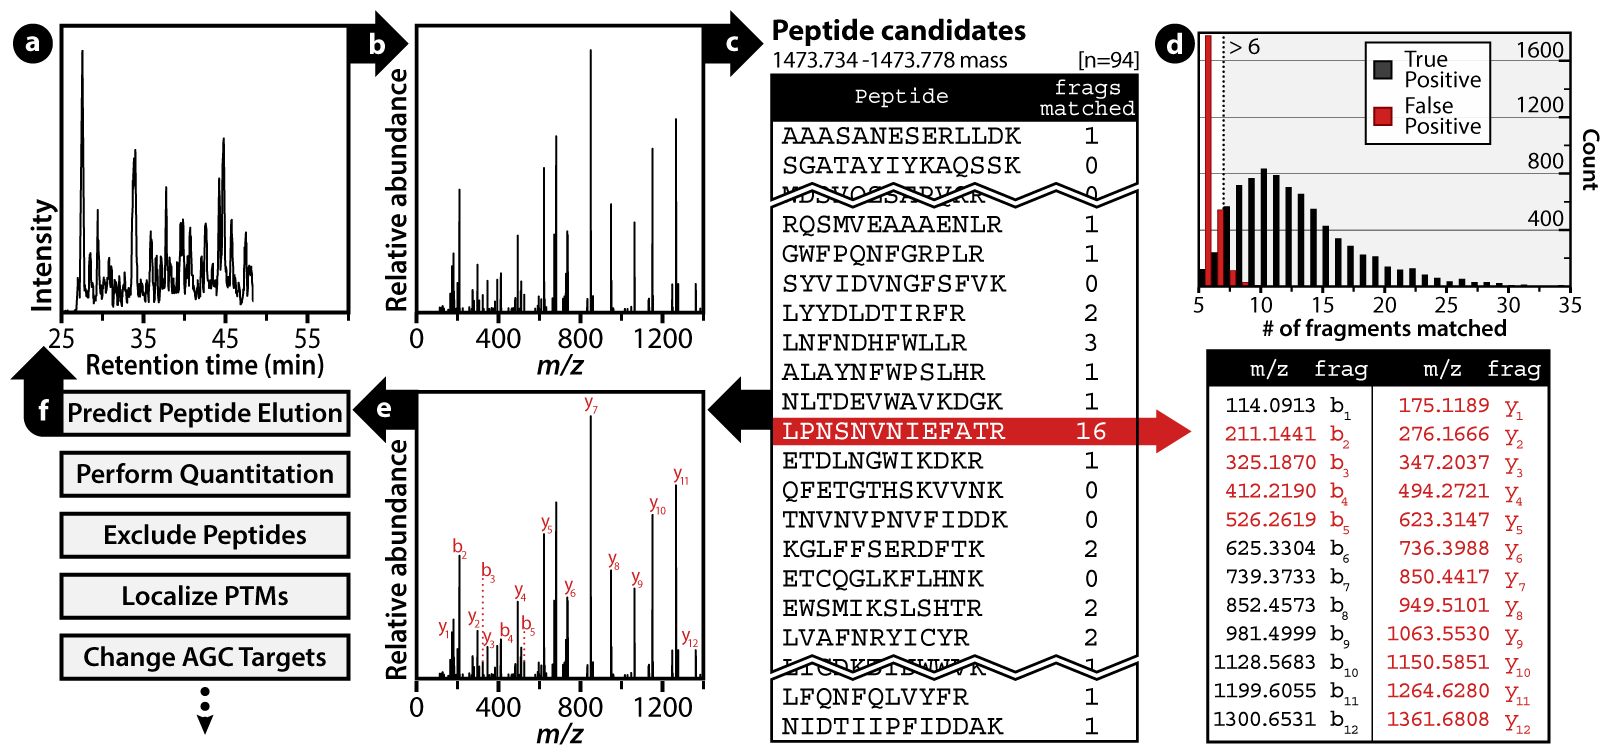
\includegraphics[width=\columnwidth]{inseq/inSeq_Fig 1.png}
	\mycaption{Progression of \inseq{} logic}{(A) A nHPLC-MS/MS chromatogram at 48.35 minutes along with an MS/MS scan (B) that was acquired at that time following dissociation of a +2 feature of \mz{} 737.86. Upon collection of the MS/MS scan, \inseq{} groups all peptide candidates (\emph{in silico}, n = 94) whose theoretical mass are within 30 ppm of the experimentally determined precursor neutral mass 1473.756 (C). Then \inseq{} performs \emph{in silico} fragmentation to produce a theoretical product ion series for each of the 94 candidates and proceeds to compare each to the experimental spectrum (<10 ppm mass accuracy). (D) Plot of \inseq{} identifications compared to conventional post-acquisition searching. \inseq{} agrees (True Positive) >98\% of the time when >6 fragment ions are matched.}
	\label{fig:inseq1}
\end{sidewaysfigure} 
The embedded peptide database-matching algorithm processes MS/MS scans immediately (Figure \ref{fig:inseq1}A\&B) by comparing product ions present in the MS/MS scan to those from peptide candidates pre-loaded onto the instrument's firmware. Note the candidate sequences are first filtered so that only sequences whose mass is within a small window (e.g., 5-50 ppm) of the sampled precursor neutral mass are considered (Figure \ref{fig:inseq1}C). For each candidate sequence the number of +1 product ions (+2 ions are included for precursors >+2) that matched the spectrum at a mass tolerance < 10 ppm is recorded (Figure \ref{fig:inseq1}C). Next, it uses straightforward scoring metrics, providing sufficient evidence for the confirmation of a putative sequence without burdening the system with non-essential calculations. On both MS platforms the real-time confirmation algorithm was expediently executed and required no hardware modification, taking an average of 16 ms to perform (Q Exactive, Figure \ref{fig:inseqs1}).
\begin{figure}[p]
	\centering
	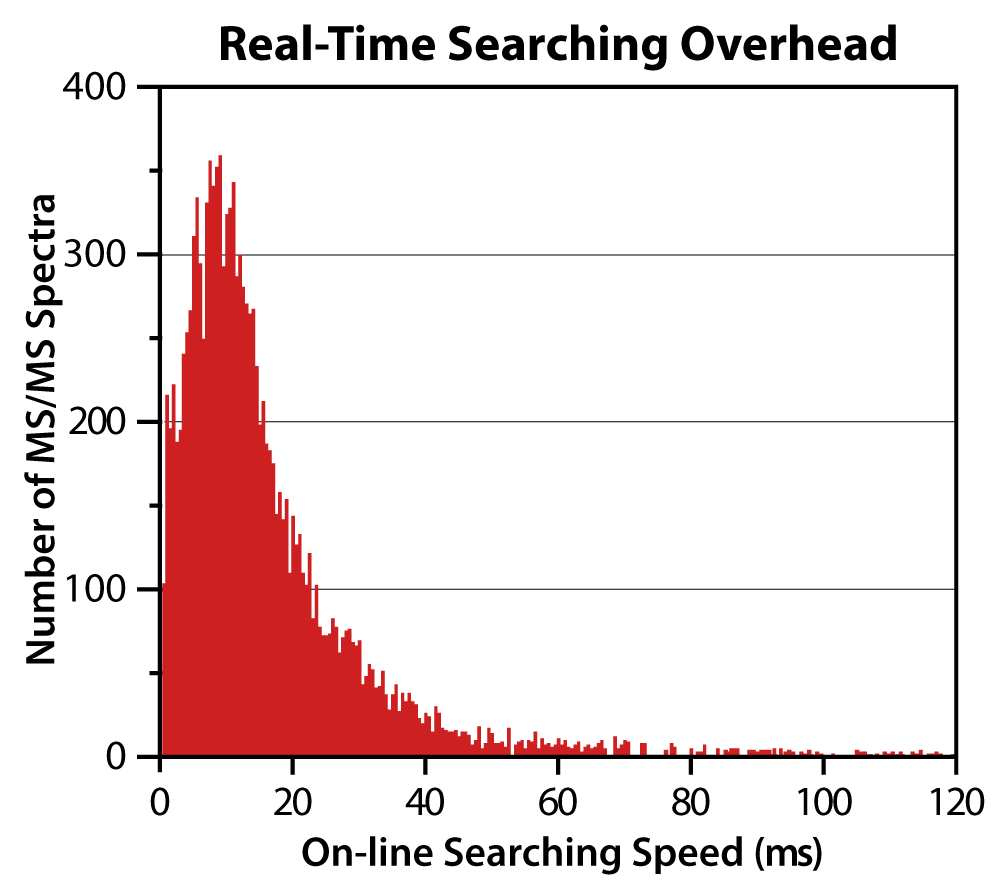
\includegraphics[width=\columnwidth]{inseq/inSeq_Fig S1.png}
	\mycaption{Distribution of \inseq{} analysis times (Q Exactive)}{The complete yeast proteome (6,717 proteins) was digested \emph{in silico}, trypsin specificity up to 3 missed cleavages) and the resulting peptides sorted to only retain those between 6-50 residues in length for a database of 1,174,780 unique sequences. The overhead accrued by \inseq{} is small ($\mu$ = 16 ms / spectrum) compared to the overall acquisition rate (\textasciitilde100-250 ms/spectrum), with over 95\% of the MS/MS events taking less than 45 ms to search.}
	\label{fig:inseqs1}
\end{figure}
To confirm that this small overhead does not affect the overall duty cycle, we compared the number of MS/MS scans performed when \inseq{} was and was not operating (9,076 DDA vs. 8,908 DDA with \inseq{}, \textasciitilde1.6\%). The number of MS scans for the peptide IVGIVSGELNNAAAK within its elution profile further demonstrates the negligible impact on duty cycle as 20 MS scans were taken with \inseq{} inactive as compared to 19 scans with \inseq{} active (Figure \ref{fig:inseqs2}).
\begin{figure}[p]
	\centering
	
\includegraphics[width=\columnwidth]{inseq/inSeq_Fig S2.png}
	\mycaption{Frequency of MS scans with and without \inseq{} active}{The extracted ion chromatograms of a random peptide (IVGIVSGELNNAAAK) is displayed for two data-dependent top 10 experiments without (top) and with (bottom) \inseq{} active. In both cases, a large number of MS scans are performed within the elution profile (20 and 19 for \inseq{} off and on, respectively).}
	\label{fig:inseqs2}
\end{figure}

To characterize the \inseq{} algorithm we performed a nHPLC-MS/MS experiment on tryptic peptides derived from human embryonic stem cells. A database consisting of all theoretical tryptic peptides (up to three missed cleavages, 6-50 in length) contained within the human proteome was uploaded to the instrument's (Q Exactive) on-board computer. A DDA method was employed and analysis proceeded as usual, except following each MS/MS scan the \inseq{} algorithm was executed and the results logged. This manifest of instant identifications was then compared to those made post-acquisition via traditional database searching at a 1\% FDR (target-decoy method). We assumed the conventional post-acquisition approach to represent the true answer and compared the number of correct instant spectral identifications as a function of matched product ions (Figure \ref{fig:inseq1}D). From these data we conclude the detection of >6 product ions at high mass accuracy (<10 ppm) by the \inseq{} algorithm produces the correct sequence identification >98\% of the time. To determine the impact of \inseq{} on the depth of protein coverage, we compared OMSSA identifications with \inseq{} identifications (species with >6 matching peaks) (Figure \ref{fig:inseqs3}). Traditional post-acquisition searching identified more peptides than \inseq{} (11,095 vs. 7,910, respectively) indicating strong initial performance but also room for further development of a more sophisticated real-time scoring algorithm.
\begin{sidewaysfigure}[p]
	\centering
	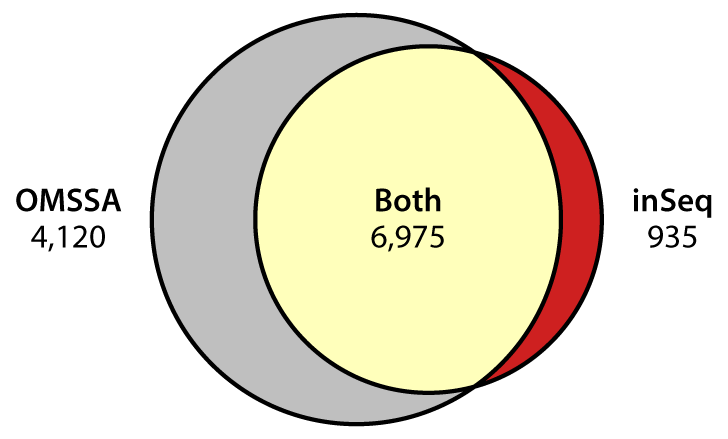
\includegraphics[width=\columnwidth]{inseq/inSeq_Fig S3.png}
	\mycaption{Overlap of \inseq{} and OMSSA identifications}{Each spectrum in a 120 min nHPLC-MS/MS gradient was scored with OMSSA and \inseq{}. OMSSA identifications were filtered to 1\% FDR and \inseq{} identifications were confirmed only if the spectra contained >6 matching peaks, as described in the text. Overlap between OMSSA and \inseq{} demonstrates that \inseq{} identifications are usually correct. The OMSSA-only identifications represent a subset of spectra which are false negatives with respect to \inseq{}.}
	\label{fig:inseqs3}
\end{sidewaysfigure}

\inseq{} represents a straightforward approach to correlate sequence to spectrum and is positioned to become an essential technology in transforming the current passive data collection paradigm. Specifically, learning the identity of a peptide that is presently eluting into the MS system permits an ensemble of advanced, automated decision-making logic. These concepts build upon our previous development of the data-dependent decision tree (DT) method. There we embedded an on-board algorithm to make unsupervised, real-time decisions of which fragmentation method to engage, based on precursor charge (\textit{z}) and \mz{}. Here, with the \inseq{} instant identification algorithm, we extend our simple DT method by adding several new decision nodes (Figure \ref{fig:inseqs4}). These nodes enable automated functionalities including: real-time elution prediction, advanced quantification, PTM localization, large-scale targeted proteomics, and increased proteome coverage, among others (Figure \ref{fig:inseq1}F).

\begin{figure}[p]
	\centering
	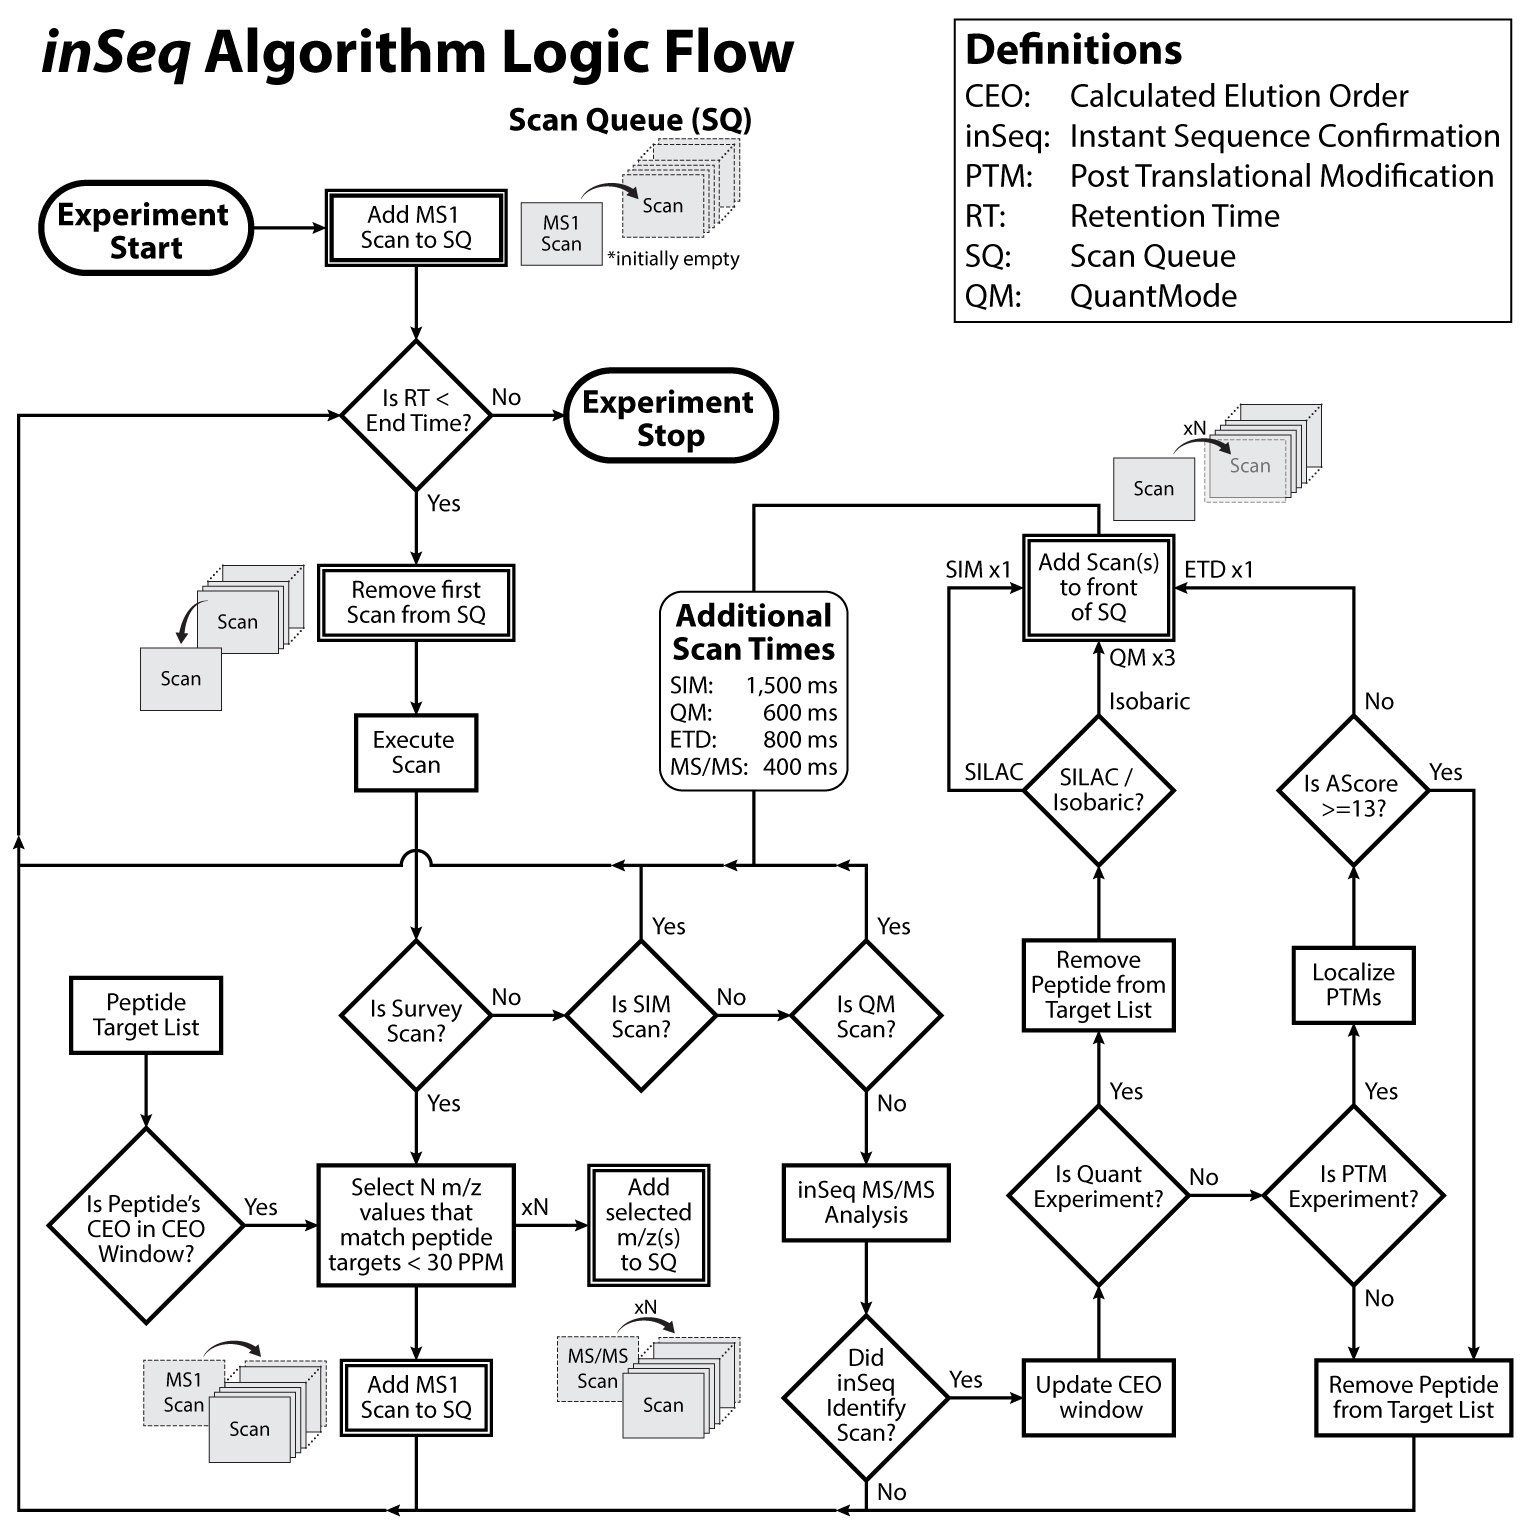
\includegraphics[width=\columnwidth]{inseq/inSeq_Fig S4.png}
	\mycaption{Basic information flow for implementing \inseq{}}{The flow of \inseq{} follows a targeted Top-N inclusion list (Target List) routine with additional analysis steps interspersed. Following an MS scan, the top 10 peaks that match precursors in the Target List (filtered by elution order) are added to a Scan Queue (SQ). Each MS/MS scan is analyzed with \inseq{} to determine if the peptide of interest is there. If identified, the peptide is removed from the Target List and additional analyses for quantitation and PTM localization may be performed.}
	\label{fig:inseqs4}
\end{figure}

\subsection*{Predicting peptide elution.}

Liquid chromatography is the conventional approach to fractionate highly complex peptide mixtures prior to measurement by MS. The highest MS sensitivity is achieved when one tunes the MS system to detect a given target (i.e., execute MS/MS) regardless of its presence in the preceding MS event (i.e., selected reaction monitoring). SRM measurements deliver both sensitivity and reproducibility at the cost of bandwidth. Specifically, if one does not know the elution time of a target, the duration of the nHPLC-MS/MS analysis must be dedicated to conditions for that specific entity. If elution times are known, then multiple SRM scan events can be programmed allowing for detection of multiple targets; however, chromatographic conditions must remain identical or the scheduled SRM elution windows will no longer align. Still, the bandwidth of that approach is low (\textasciitilde100 peptide targets per nHPLC-MS/MS analysis) and compiling such an experiment is highly laborious.\cite{indexion}

We surmised that \inseq{} could inform the MS system, without human intervention, of which peptide targets are most likely to subsequently elute. Such capability could enable robust, large-scale targeting (>500 per analysis) in an automated manner. Our approach relies upon relative peptide elution order and, consequently, bypasses the use of absolute retention times, which shift depending on chromatographic conditions and are not directly portable from multiple disparate experiments. Peptide elution order can be obtained in two ways: First, discovery experiments can be employed to determine retention order by normalizing the measured retention time for each detected peptide sequence. Second, the relative hydrophobicity for any sequence can be theoretically determined using existing software (e.g., SSRCalc).\cite{ssrcalc1,ssrcalc2,incselect} In our experience experimentally determined retention order offers better precision; still, it requires prior knowledge which may not be available. However retention order is determined, the real-time confirmation algorithm maintains a rolling average of the calculated elution order (CEO---a number describing the relative elution order of a target peptide) so that target peptides having nearby CEOs are specifically pursued (Figure \ref{fig:inseq1}B).
\begin{sidewaysfigure}[p]
	\centering
	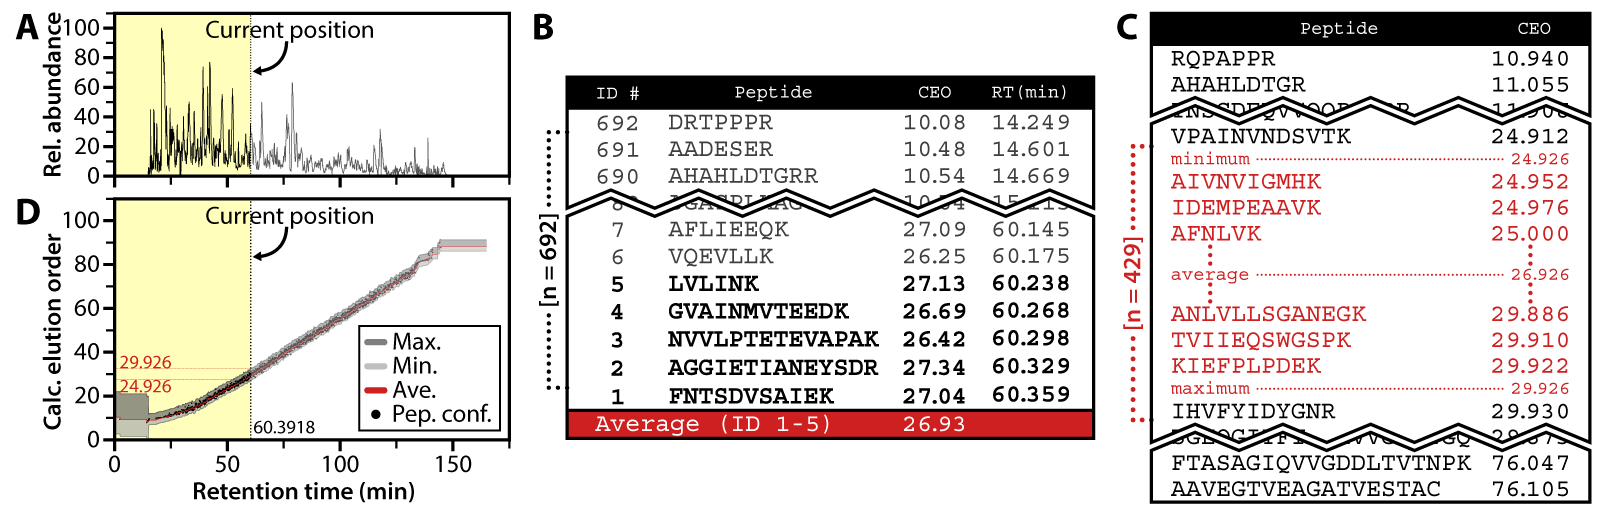
\includegraphics[width=\columnwidth]{inseq/inSeq_Fig 2.png}
	\mycaption{Elution order prediction using \inseq{}}{(A) Experimental chromatogram, 60.39 minutes into a 120 minute gradient, obtained while \inseq{} was recording instant identifications. (B) The \inseq{} calculated elution order (CEO) obtained by averaging the CEOs of the preceding 5 instantly identified peptides. (C) The asymmetric window (5 a.u.) surrounding the instant CEO average ($\mu$ = 26.926) and their corresponding sequences. (D) This analysis is repeated following each new peptide confirmation to constantly realign the CEO window based on current chromatographic conditions.}
	\label{fig:inseq2}
\end{sidewaysfigure}
Figure \ref{fig:inseq2} presents an overview of this approach. This example, 60.39 minutes into the chromatograph, highlights the last five \inseq{} identified peptides and their average CEO (26.926 a.u.). The on-board algorithm then computes an asymmetric CEO window (5 a.u., 24.926-29.926) that presents a short list of desired targets having CEOs within that range (Figure \ref{fig:inseq1}C). With this information the MS system can trigger specialized MS/MS scans specific to this refined target subset. Note that as targets are identified, the CEO window is dynamically adjusted so targets come into and out of the range precisely when they are eluting.

To test this technology, we performed a DDA nHPLC-MS/MS experiment in which tryptic peptides from a human ES cell sample were separated over a 60 minute gradient. Following data collection the resulting MS/MS spectra were mapped to sequence using database searching (1\% FDR). The unique peptide identifications (4,237) were sorted by observed retention time---this ordering then served as the CEO. 3,000 of these peptides were randomly selected as ''targets'' and loaded onto the instrument firmware (Velos-Orbitrap), along with their respective CEO, as a database for \inseq{}. The sample was then re-analyzed with \inseq{} activated, but with a doubled gradient length (120 min). Figure \ref{fig:inseq2}D displays the CEO window as calculated in real-time by the MS system (\inseq{}) plotted beside the actual elution time of identified peptides. Greater than 95\% of the peptides (2,889) fell within the rolling CEO window and were identified by both \inseq{} and post-acquisition searching. At our present capability we can achieve window widths similar to those used in absolute scheduling type experiments (\textasciitilde3-6 minutes) on a scale that is 30X larger (e.g., 3,000 targets vs. 100) with minimal effort.\cite{indexion,integrated} Further, we demonstrate that our approach adapts to different chromatographic conditions with no negative effects (Figure \ref{fig:inseq2}D). The key to the high portability and simplicity of our algorithm is the use of \inseq{} for continual, real-time realignment.

\subsection*{Improvement of quantitative accuracy.}

The method of stable isotope labeling has greatly propelled large-scale, quantitative analysis.\cite{pheromone,8plex,haploid,7tmr,esips,leeyeast} While generally robust, these techniques can yield spotty data for certain peptide and protein groups---mainly those present at low abundances. For SILAC, low signal-to-noise (S/N) precursor peaks in the MS scan often result in either omission of that particular feature or quantitative imprecision, if included.\cite{dynamicrange} For isobaric tagging, low intensity reporter ion signals (MS/MS) induce similar shortcomings.\cite{itraqerror} We surmised that \inseq{} could be employed to counter these limitations.

First, we developed an \inseq{} module to improve the quality of isobaric label-based measurements. The module analyzes MS/MS spectra, using \inseq{}, and, when a peptide of interest is detected, the quality of quantitative data is assessed. Should the reporter ion signals fall below a specified threshold, \inseq{} triggers follow-up scans to generate increased signal at the very instant the target peptide is eluting. In one implementation, we instructed \inseq{} to automatically trigger three quantitative scans, using the recently developed QuantMode (QM) method, to generate superior quality quantitative data on targets of high value.\cite{quantmode} The trio of QM scans are then summed offline.

To assess this decision node we analyzed a sample comprising three biological replicates of human embryonic stem cells pre- and two days-post bone morphogenetic protein 4 (BMP4) treatment (i.e., TMT 6-plex, three pre-treatment and three post BMP4 treatment cell populations). BMP4, a growth factor that induces context-dependent differentiation in pluripotent stem cells, is widely used to study differentiation to biologically relevant cell lineages such as mesoderm and endoderm.\cite{bmp,kdr,nanog} Whenever a target peptide was identified by \inseq{}, three QM scans were immediately executed. This ensured that all identified peptides had the same number of quantitation scans, enabling a direct comparison for analyzing multiple QM scans within this experiment.
\begin{sidewaysfigure}[p]
	\centering
	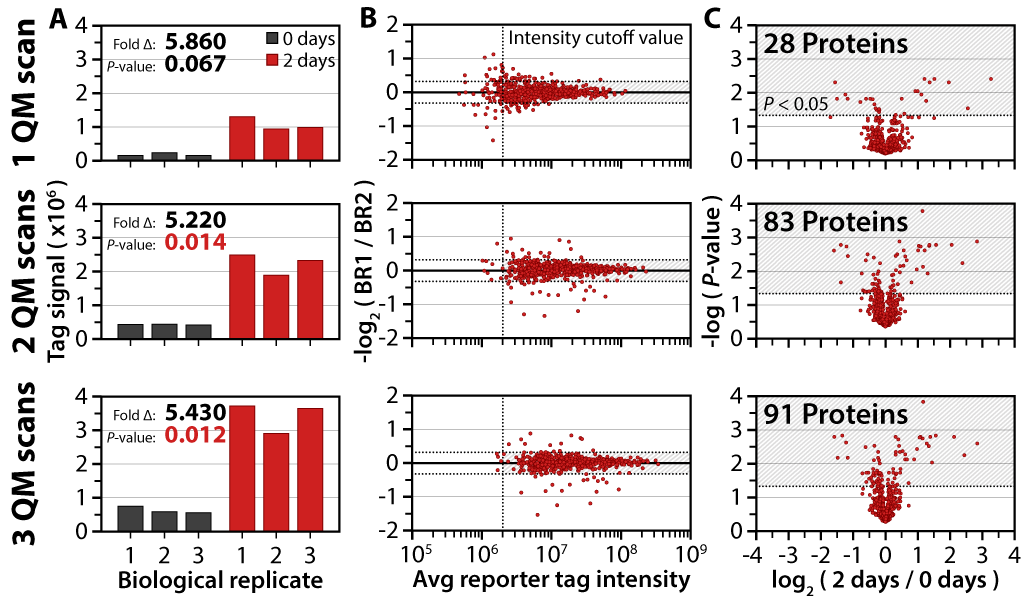
\includegraphics[width=\columnwidth]{inseq/inSeq_Fig 3.png}
	\mycaption{\inseq{} improves quantitative outcomes for isobaric tagging}{An \inseq{} decision node was written so that a real-time identification of a target sequence prompted automatic acquisition of three consecutive QuantMode (QM) scans. (A) Summing the reporter ion tag intensity from one, two, or three QM scans greatly improves the statistical significance of the measurement. (B) Summation of QM technical replicates reduces the variation in biological replicate measurement by increasing reporter ion S/N. (C) \inseq{}-triggered QM scans increase the number of significantly changing proteins from 28 to 91.}
	\label{fig:inseq3}
\end{sidewaysfigure}
Figure \ref{fig:inseq3}A demonstrates the benefit of summing isobaric tag intensities from one, two, or three consecutive quantitation scans for an \inseq{} identified target peptide having the sequence FCADHPFLFFIR from the protein SERPINB8. Here the ratio of change between control and treatment cell lines measured in one QM scan is large (5.86) but not significant (P = 0.067, Student's t-test with Storey correction).\cite{storey} Note significance testing was accomplished by assessing variation within the three biological replicates of both treatment and control cell lines. The measured ratio remains relatively unchanged (5.22 and 5.43) as reporter tag signals from additional quantitation scans are added; however, the corresponding P-values decrease to 0.014 and 0.012 when two or three quantitation scans are summed. By plotting the $\log_2$ ratio of quantified proteins from the three biological replicates against the average intensity of isobaric labels (Figure \ref{fig:inseq3} B) we demonstrate this improved significance results from boosted reporter S/N. Ideally this $\log_2$ ratio would be zero, indicating perfect biological replication; however, when only one quantitation scan is employed this ratio severely deviates from zero with decreasing tag intensity. To improve overall data quality and to omit potentially erroneous measurements we, and others, employ arbitrary reporter signal cutoffs (dashed vertical line in Figure \ref{fig:inseq3}B). Summation of additional quantitation scans increases the average reporter tag intensity, raising nearly all of the protein measurements above the intensity cutoff value (74, 9, and 4 proteins omitted using one, two, and three quantification scans, respectively). This quantification decision node also increased the number of proteins within 25\% of perfect biological replication (horizontal dashed line).

To determine if the method could improve the number of statistically significant differences between the cell populations, we calculated the $\log_2$ ratio of treated vs. control (i.e., 2 days/0 days) for each of the 596 quantified proteins (P<0.05, Student's t-test with Storey correction, Figure \ref{fig:inseq3}C). Only 28 proteins display significant change when one QM scan is used. By simply adding the reporter tag signal from additional scans the number of significantly changing proteins increases nearly threefold, from 28 to 91 when all three QM scans are analyzed together.
Many stable isotope incorporation techniques measure heavy and light peptide pairs in MS (e.g., SILAC). This approach, of course, requires the detection of both partners; note low abundance peptides are often identified with low, or no, precursor signal in the MS. We supposed that addition of another \inseq{} decision node could circumvent this problem. We cultured human embryonic stem cells in light and heavy media. Protein extract from these cultures was mixed 5:1 (light:heavy), before digestion overnight with LysC. The SILAC node was developed to select precursors from an MS scan only if the monoisotopic mass was within 30 ppm of any target on a list which contained 4,000 heavy and light peptides from a previous discovery run. Targets were selected only if the SILAC ratio deviated from the expected ratio of 5 by 25\%, i.e., the subset containing the most error. Following MS/MS, the resulting spectra were analyzed using \inseq{}. When a target of interest was identified, \inseq{} instructed the system to immediately record a SIM scan surrounding the light/heavy pair with a small, charge-dependent isolation window (\textasciitilde8-10 Th).

The average ratio of the light and heavy peptides subtly, but significantly, shifted from 4.47 under normal analysis to 5.34 for the \inseq{} triggered SIM scans (Student's t-test, p-value < 6\e{-20}). More importantly, the number of useable measurements, i.e., when both partners of the pair are observed, increased by \textasciitilde20\% (2,887 under normal analysis to 3,548 with \inseq{}, Figure \ref{fig:inseqs5}A).
\begin{sidewaysfigure}[p]
	\centering
	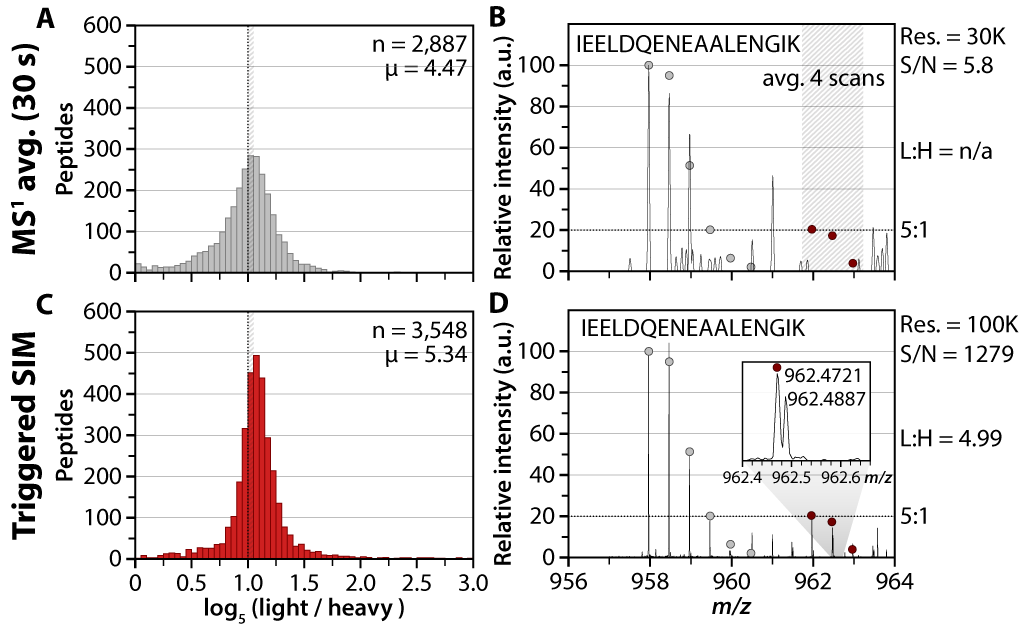
\includegraphics[width=\columnwidth]{inseq/inSeq_Fig S5.png}
	\mycaption{\inseq{} can improve quantitative outcomes for SILAC}{Following an \inseq{} confirmation of a peptide having the sequence, IEELDQENEAALENGIK, a narrow (8 Th), high-resolution (R = 100,000) SIM scan was automatically triggered and increased the S/N from 5.8 to 1,279 (Panels A and B). This SIM scan enabled detection of both partners and yielded the correct ratio of 5:1 (light:heavy). Besides increased dynamic range, the theoretical isotope distribution (shown in open circles) closely matches in the SIM scan (B), while the signal for the heavy partner is not even detectable in the MS (A). Over our entire data set, the \inseq{} triggered SIM scans improved the mean ratio from 4.47 to 5.34, but, more impressively, produced \textasciitilde20\% more quantifiable measurements (3,548 vs. 2,887).}
	\label{fig:inseqs5}
\end{sidewaysfigure}
Figure \ref{fig:inseqs5}B displays an example of the \inseq{}-triggered SIM scan and the increase in S/N and accuracy it affords. Here the MS/MS scan of the light partner was mapped, in real-time, to the sequence IEELDQENEAALENGIK. This event triggered a high resolution SIM scan (8 Th window), which led to the ratio of 4.99:1 (correct ratio 5:1). Here gas phase enrichment was essential to quantify the relative abundance, as the isotopic envelope of the heavy partner was not observed, even with extensive spectral averaging of successive MS scans (\textasciitilde30 s, Figure \ref{fig:inseqs5}B). Whether for MS or MS/MS centric methods, we conclude that \inseq{} technology will significantly improve the quality of quantitative data with only a minimal impact on duty cycle.

\subsection*{Post-Translational Modification Site Localization.}

The presence of post-translational modifications (PTMs) on proteins plays a major role in cellular function and signaling. Unambiguous localization of PTMs to residue demands observation of product ions resulting from cleavage of the residues adjacent to the site of modification, i.e., site-determining fragments (SDFs). In a typical analysis only about half of the identified phosphorylation sites can be mapped with single amino acid resolution, stymying systems-level data analysis. We reasoned that \inseq{} could be leveraged to boost PTM localization rates by dynamically modifying MS/MS acquisition conditions when necessary. As such we developed an online PTM localization decision node to determine, within milliseconds, whether a MS/MS spectrum contains SDFs to unambiguously localize the PTM. Should SDFs be lacking, \inseq{} instantly orchestrates further interrogation.

The PTM localization node is engaged when \inseq{} confirms the detection of a PTM-bearing peptide. After the sequence is confirmed, \inseq{} assesses the confidence with which the PTM(s) can be localized to a particular amino acid residue. This procedure is accomplished by computing an online probability score similar to post-acquisition PTM localization software---i.e., AScore.\cite{ascore} Briefly, \inseq{} compares all possible peptide isoforms against the MS/MS spectrum. For each SDF the number of matches at <10 ppm tolerance is counted and an AScore is calculated (\inseq{} uses similar math). If the AScore of the best fitting isoform is above 13 (p < 0.05) the PTM is declared localized. When the AScore is below 13, however, \inseq{} triggers further characterization of the eluting precursor until either the site has been deemed localized or all decision nodes have been exhausted. Additional characterization can include many procedures such as acquisition of MS/MS spectra using different fragmentation methods (e.g., CAD, HCD, ETD, PD, etc.), varied fragmentation conditions (e.g., collision energy, reaction time, laser fluence, etc.), increased spectral averaging, MSn, pseudo MSn, modified dynamic exclusion, and altered AGC target values, among others.\cite{neutralloss}
\begin{figure}[p]
	\centering
	
\includegraphics[width=0.6\columnwidth]{inseq/inSeq_Fig 4.png}
	\mycaption{\inseq{} can improve PTM localization rates}{Following MS/MS (HCD) of the singly-phosphorylated precursor RNsSEASSGDFLDLK, \inseq{} could not find sufficient information to confidently localize the modification to either Ser 3 or 4 (A, AScore = 0). \inseq{} immediately triggered an ETD MS/MS scan event on the same precursor (B). This spectrum was assigned an AScore of 31.0129 (phosphorylation on Ser3) and was considered confidently localized---note the SDFs $c_3$ and $z\cdot_{12}$ ions. (C) Globally, the \inseq{} localization calculation agreed with offline analysis using the actual AScore algorithm. (D) Using a simple dissociation method DT, \inseq{} produced a confidently localized phosphorylation site for 78 of 324 unlocalizable sites, saving nearly 25\% of them.}
	\label{fig:inseq4}
\end{figure}

To obtain proof-of-concept results we wrote a simple \inseq{} node that triggered an ETD MS/MS scan of phosphopeptides that were not localized following HCD MS/MS. In one example (Figure \ref{fig:inseq4}) the sequence, RNSSEASSGDFLDLK, was confirmed to contain a phosphoryl group; however, the \inseq{} algorithm could not confidently localize the PTM to any of the four Ser residues (AScore = 0). Next, \inseq{} triggered an ETD MS/MS scan of the same precursor (Figure \ref{fig:inseq4}B). The resulting spectrum was then analyzed for the presence of the SDFs, \fragment{c}{3} / \fragment{z\cdot}{12}. Both of these fragments were present and the site was localized to Ser 3 with an AScore of 31.0129 (p < 0.00079). Post-acquisition analysis confirmed the results of our online \inseq{} approach---both spectra (HCD and ETD) were confidently identified and their calculated AScores were 0 and 45.58, respectively. When compared on a global scale, 993 of the 1,134 \inseq{}-identified phosphopeptides had localization judgments that matched post-acquisition AScore analysis (Figure \ref{fig:inseq4}). This slight difference is the result of using different localization algorithms for online and post-acquisition analysis. Primarily, the post-acquisition method considers fragment ions on either side of the site-determining fragments separately, while the \inseq{} method does perform this extra step for simplicity.\cite{esips,ascore} These data demonstrate that our localization node is highly effective at instantaneously determining whether a PTM site can be localized. Unfortunately, only marginal gains were achieved in this basic implementation as most precursors were doubly charged and, therefore, not effectively sequenced by ETD. Next, we modified the \inseq{} decision node to incorporate a dissociation method DT. Here a follow-up ETD or combination ion trap CAD/HCD scan was triggered depending upon precursor charge (\textit{z}) and \mz{}. With the slightly evolved algorithm the \inseq{} method detected 998 phosphopeptides in a single shotgun experiment. It determined that 324 of these identifications lacked the information to localize the PTM site and, in those cases, triggered the new dissociation decision node. 78 of these unlocalizable sites were confidently mapped with this technique---salvaging nearly 25\% of the unlocalized sites (Figure \ref{fig:inseq4}D). These encouraging results demonstrate that \inseq{} has great promise to curtail the problem of PTM localization in a highly automated fashion. We note there are dozens of parameters to explore in the continued advancement of this PTM localization decision node.

\section{Conclusion}

Here we described an instant sequencing algorithm (\inseq{}) that operates using the pre-existing processors of the MS. Rapid real-time sequencing affords several novel data acquisition opportunities. To orchestrate these opportunities we constructed an advanced decision tree logic that extends our earlier use of the method to intelligently select dissociation type. The approach can circumvent longstanding problems with the conventional DDA paradigm. We provided three such examples herein. First, we demonstrated that knowledge of which peptide sequences are eluting can facilitate the prediction of soon to elute targets. This method shows strong promise to revolutionize the way in which targeted proteomics is conducted. Second, we used quantitative decision nodes that fired when \inseq{} detected a peptide sequence of interest. With either SILAC or isobaric tagging, significant gains in quantitative outcomes were documented. Third, we endowed \inseq{} with an instant PTM site-localization algorithm to determine whether or not to initiate more rigorous follow-up at the very instant the peptide of interest was eluting. We show that the \inseq{} site localizer is highly effective (90\% agreement with post-acquisition analysis) and that triggering a simple dissociation method DT can improve site localization by \textasciitilde25\%. Further development will doubtless deliver additional gains.

Targeted proteomics is an area of increasing importance. Following discovery analysis it is natural to cull the list of several thousand detected proteins to several hundred key players. In an ideal world these key proteins are then monitored in dozens or even hundreds of samples with high sensitivity and reproducibility, without rigorous method development and be expediently performed. We envision that advanced DT analysis with \inseq{} could offer such a platform. Using the retention time prediction algorithm we introduced here one can foresee the \inseq{} algorithm quickly and precisely monitoring hundreds of peptides without the extensive labor and pre-planning required by the selected reaction monitoring (SRM) technique, current state-of-the-art.\cite{srm} Other possibilities include automated pathway analysis where user-defined proteins, within a collection of pathways, are simply uploaded to the MS system. Then, \inseq{} automatically determines the best peptides to track, their retention times, and constructs the method. Two key advantages over current SRM technology make this operation possible. First, knowledge of specific fragmentation transitions are not necessary as all products are monitored with high mass accuracy. Second, precise elution time scheduling is not necessary as \inseq{} can use CEO, experimental or theoretical, to dynamically adjust the predicted elution of targets. In this fashion the most tedious components of the SRM workflow can be avoided.

\section{Experimental Methods}

\subsection{Cell Culture.}
Human embryonic stem cells (line H1) were maintained in feeder independent media as previously described.\cite{feeder} For SILAC experiments, DMEM/F12 lacking lysine and arginine (Mediatech Inc.) was supplemented with light arginine (Sigma-Alrich) and either heavy labeled lysine (Cambridge Isotopes Laboratories) or light lysine (Sigma-Aldrich). Cells were cultured on Matrigel (BD Biosciences) and split 1:8 at approximately 80\% confluency using 0.1 mM EDTA. To harvest cells, TripLE Express (Invitrogen) was applied for five minutes at 37$^\circ$C. Following cell detachment, an equivalent volume of ice-cold DPBS (Invitrogen) was added before centrifugation. Cell pellets were subsequently washed twice in ice-cold DPBS and stored at $-80^\circ$C. BMP4-treated cells were grown and harvested as described above, except that 5 ng/mL BMP4 (R\&D Systems) was added into the media and cells were split using TrypLE (Invitrogen). For BMP4 experiments, single cells were plated at the density of 4\e{4}/cm$^2$, for 2 days of treatment. We collected \textasciitilde$10^8$ cells for each analysis.

\subsection{Cell Lysis.}
For all analysis, human embryonic stem cells were lysed in ice-cold 8 M urea, 40 mM NaCl, 50 mM tris (pH 8), 2 mM MgCl$_2$, 50 mM NaF, 50 mM $\beta$-glycerol phosphate, 1 mM sodium orthovanadate, 10 mM sodium pyrophosphate, 1X mini EDTA-free protease inhibitor (Roche Diagnostics), and 1X phosSTOP phosphatase inhibitor (Roche Diagnostics). To solubilize protein and ensure complete lysis, samples were sonicated three times for 15 seconds with 30 second pauses. Total protein was then quantified using a BCA protein assay kit (Thermo Scientific Pierce).

\subsection{Isobaric Label Sample Preparation.}
For analysis, 250 $\mu$g of protein from each sample was reduced by adding DTT to a final concentration of 5 mM, and alkylated with 15 mM iodoacetamide before final capping with 5 mM DTT. Digestion was carried out by adding LysC (Wako Chemicals) at a 1:100 enzyme-to-protein ratio and incubating at 37$^\circ$C for 2 hours. At this time, the lysate was diluted with 25 mM tris (pH 8) to a final urea concentration of 1.5 M and further digested for 12 hours at 37$^\circ$C with trypsin (Promega) at a 1:100 enzyme to protein ratio. Peptides were then acidified with TFA to quench the reaction and de-salted using C-18 solid phase extraction (SPE) columns (Waters). TMT labeling was carried out per manufacturer's directions (Thermo Scientific Pierce). Samples were mixed in a 1:1:1:1:1:1 ratio before analysis.

\subsection{SILAC Sample Preparation.}
Protein from the light and heavy embryonic stem cell cultures was mixed in a 5:1 ratio (light:heavy) by pooling 2.5 mg of light protein and 0.5 mg of heavy protein. The sample was reduced by adding DTT to a final concentration of 5 mM, and alkylated with 15 mM iodoacetamide before final capping with 5 mM DTT. Digestion was carried out by adding LysC (Wako Chemicals) at a 1:100 enzyme-to-protein ratio and incubating at 37$^\circ$C overnight. Peptides were then acidified with TFA to quench the reaction and de-salted using C-18 solid phase extraction (SPE) columns (Waters).

\subsection{Phosphopeptide Sample Preparation.}
From an embryonic stem cell culture, 1 mg of protein was reduced by adding DTT to a final concentration of 5 mM, and alkylated with 15 mM iodoacetamide before final capping with 5 mM DTT. Digestion was carried out by adding LysC (Wako Chemicals) at a 1:100 enzyme-to-protein ratio and incubating at 37$^\circ$C for 2 hours. At this time, the lysate was diluted with 25 mM tris (pH 8) to a final urea concentration of 1.5 M and further digested for 12 hours at 37$^\circ$C with trypsin (Promega) at a 1:100 enzyme to protein ratio. Peptides were then acidified with TFA to quench the reaction and de-salted using C-18 solid phase extraction (SPE) columns (Waters).
Phosphopeptides were enriched via immobilized metal affinity chromatography (IMAC) using magnetic beads (Qiagen). Following equilibration with water, the beads were treated with 40 mM EDTA (pH 8.0) for 30 minutes with shaking, and washed 3X with water again. The beads were then incubated with 100 mM FeCl$_3$ for 30 minutes with shaking and finally were washed 3 times with 80\% acetonitrile/0.1\% TFA. Samples were likewise resuspended in 8\% acetonitrile/0.15\% TFA and incubated with beads for 45 minutes with shaking. The resultant mixture was washed 3 times with 1 mL 80\% acetonitrile/0.1\% TFA, and eluted using 1:1 acetonitrile:0.7\% NH$_4$OH in water. Eluted phosphopeptides were acidified immediately with 4\% formic acid and lyophilized to \textasciitilde5 $\mu$L.

\subsection{nano-High Performance Liquid Chromatography.}
For all samples online reverse-phase chromatography was performed using a nanoACQUITY UPLC system (Waters). Peptides were loaded onto a pre-column (75 $\mu$m ID, packed with 7 cm C18 particles, Alltech) for 10 min at a flow rate of 1 $\mu$L/min. Samples were then eluted over an analytical column (50 $\mu$m ID, packed with 15 cm C18 particles, Alltech) using either a 60 or 120 min linear gradient from 2\% to 35\% acetonitrile with 0.2\% formic acid and a flow rate of 300 nL/min.

\subsection{Target List Construction and \inseq{} Setup.}
For all experiments, the monoisotopic mass, charge state, and previously determined retention time of target peptides was included for use by the \inseq{} algorithm. In addition, peptides modified on methionines or tyrosines were omitted from all target lists. For peptide elution and isobaric label quantitation \inseq{} experiments, a target list of 4,000 peptides was constructed from a previous nHPLC-MS/MS experiment employing a 90 min nHPLC gradient. For SILAC \inseq{} experiments, peptides identified at 1\% FDR in a discovery nHPLC-MS/MS experiment were analyzed to determine the light:heavy partner ratio. A target list of 2,000 peptide pairs (4,000 total peptides) whose ratio deviated from the expected value of 5 by at least 25\% was constructed. This subset of peptides included many measurements in which the signal to noise was low, or a partner was missing. For phosphorylation \inseq{} experiments, phosphopeptides identified at 1\% FDR in a discovery nHPLC-MS/MS experiment were analyzed by the Phosphinator localization software to assign phosphosite locations. A target list comprising 2,174 phosphopeptides was constructed and used for both ETD only and decision tree (DT) \inseq{} methods.

Target lists were loaded into the instrument's firmware for instant access during acquisition. Peptide lists were stored in an internal database and sorted based on their precursor mass for fast look ups using a binary search algorithm. A parameter file was preloaded into the firmware prior to each experiment to specific scan sequences and instrument parameters needed for the intended experiment.

\subsection{Mass Spectrometry.}
All experiments were performed on Thermo LTQ Orbitrap Velos and Q Exactive mass spectrometers. The LTQ Orbitrap Velos used firmware version 2.6.0.1065 SP3 with additional ion trap control language (ITCL) modifications to enable \inseq{} operation. MS scans were performed in the Orbitrap at 30,000 resolution at a max injection time of 500 ms and a target value of 1e6. MS/MS scans were also performed in the Orbitrap at a resolution of 7,500 and with HCD normalize collision energy (NCE) of 27\%, for a max fill time of 500 ms. The Q Exactive was operated using version 2.0 Build 142800 with a modified python code base for \inseq{} data acquisition control. Q Exactive MS scans were collected at 70,000 resolution for a max injection time of 120 ms or if the 1e6 AGC target value was reached. MS/MS events were measured at 17,500 resolution at a target value of 1e5, 120 ms max injection time and 26\% NCE. Instrument methods for both the LTQ Orbitrap Velos and Q Exactive were overridden during acquisition by the instrument's firmware to provide for dynamic \inseq{} operation. Processing times for \inseq{} were similar on the older Velos-Orbitrap system with the newer Q Exactive; however, a \textasciitilde100 ms overhead was included because complete collection of the Orbitrap transient signal is necessary before the spectrum can be examined.

\subsection{Database searching and FDR estimation.}
MS/MS data was analyzed using the Coon OMSSA Proteomics Software Suite (COMPASS).\cite{compass} The Open Mass Spectrometry Search Algorithm (OMSSA; version 2.1.8) was used to search spectra against the International Protein Index(IPI) human database version 3.85.\cite{omssa} For all experiments, carbamidomethylation of cysteines was included as a fixed modification, while oxidation of methionines was set as a variable modification. For TMT experiments, TMT on the N-terminus and TMT on lysines were included as fixed modifications and TMT on tyrosines was added as a variable modification. For SILAC experiments heavy lysine was added as a variable modification. Precursor mass tolerance was set to $\pm$4.5 Da and monoisotopic mass tolerance was set to $\pm$0.015 Da for fragment ions. Results were filtered to a 1\% FDR at both the peptide and protein level with a maximum precursor mass error of 50 ppm. For phosphopeptides, the Phosphinator software was used to localize phosphorylation sites.\cite{esips}

\subsection{Protein and Peptide Quantification.}
TMT quantification was performed using TagQuant within COMPASS. This program extracts reporter ion intensities and multiplies them by injection times to determine counts. Purity correction was performed as previously described.\cite{itracker} Tag intensities were normalized to ensure that the total signal from each channel was equal. For evaluation of multiple QuantMode (QM) scans, data was analyzed at the peptide level by only quantifying the first, the sum of first and second, or the sum of the first, second, and third QM scans using TagQuant. Peptides were then combined into protein groups (ProteinHerder) and quantified at the protein level (ProteinTagQuant) within COMPASS. Experimental ratios and p-values (Student's t-test assuming equal variance) were determined using Microsoft Excel. To correct for multiple hypothesis testing, we applied Storey correction using the freely available program QVALUE.\cite{storey}
SILAC quantification was performed with in-house software that retrieved the peak intensities of both SILAC partners from either a single \inseq{}-triggered SIM scan (monoisotopic peak) or performed an extracted ion chromatogram (30 sec window) of identified precursor. A ratio of partner abundance was only calculated if both SILAC partners had an intensity at least twice that of the noise.

\bibliographystyle{ieeetr}
\bibliography{inseq}

